A szoftverrendszerek tesztelése egy nagyon fontos lépés a megfelelő minőség és megbízhatóság biztosításának szempontjából. Célja minimálisra csökkenteni a hibák számát, és biztosítani, hogy a szoftver a tervezett módon működjön. Minél több használati esetet és forgatókönyvet tesztelünk le, annál hibatűrőbbnek tekinthető az adott rendszer. Emellett fontos, hogy az esetleges hibákra minél hamarabb fény derüljön, mert minél később kerülnek kijavításra, annál többe fognak kerülni. Szerencsére napjainkban már számos tesztelési keretrendszer áll rendelkezésre, amelyek segítségével egyszerűen és hatékonyan tesztelhetjük a szoftverünket, sőt már automatizálni is tudjuk ezt a folyamatot.

A projekthez tartozó felhasználói és admin weboldalak tesztelésére a Cypress\footnote{Cypress: \url{https://www.cypress.io/}} keretrendszert használtam, mivel nagyon jól integrálható a Vue keretrendszerbe. Ennek segítségével 20 különböző tesztet készítettem, amelyek összesen 65 tesztesetet fednek le. Egy teszt egy teljes funkcionalitás tesztelését jelenti, mint például a bejelentkezési folyamat, míg a teszt eset ennek egy specifikus lefutása, mint például a bejelentkezési kísérlet helytelen adatokkal. Mivel egy adott funkcionalitást általában többféleképpen lehet használni, ebből  következik, hogy egy teszt több különböző tesztesetet is tartalmazhat. A UI teszteknek két típusát különböztethetjük meg: komponens és end-to-end (végponttól-végpontig). A komponens tesztek során az egyes komponenseket teszteljük külön egységekként, míg az end-to-end tesztek során a teljes alkalmazást teszteljük, azaz a komponensekből felépített felhasználói felületet. Most pedig következzen a Cypress bemutatása és a megvalósított tesztek részletes leírása.

\section{Cypress}
A Cypress egy JavaScript alapú tesztelési keretrendszer, amely a böngészőben fut, és lehetővé teszi a felhasználói felületek tesztelését. Elérhető Windows, macOS és Linux operációs rendszerekre és támogatja a legnépszerűbb böngészőket, de rendelkezik saját beépített böngészővel is. A keretrendszer alkalmas end-to-end tesztek írására és a nagyobb JavaScript keretrendszerek esetében, mint amilyen a Vue is, komponens tesztek is futtathatóak benne. Főbb erősségei a következők:
\begin{itemize}
    \item \textbf{Időutazás:} A Cypress minden egyes lépésről képernyőképet készít és elmenti az adott időponthoz tartozó állapotot, így lehetőség van visszalépni az időben a tesztek lefutása után is.
    \item \textbf{Hálózati forgalom vezérlése:} A Cypressben lehetőség van a hálózati forgalom figyelésére és manipulálására is, így akár backend nélkül is futtathatóak a tesztek.
    \item \textbf{Kémfunkciók:} Figyelhetőek és módosíthatóak belső függvények, változók és események is a tesztek során.
    \item \textbf{Egyszerűség és hatékonyság:} A Cypress egyszerűen telepíthető és használható a Node Package Manager (NPM) által, és a tesztek gyorsan futnak, mivel a tesztelés a böngészőben történik.
\end{itemize}

\section{Megvalósított tesztek}
A weboldalak komponenseinek teszteléséhez 5 komponens tesztet készítettem, amelyek a térképet és a különböző listaelemeket tesztelik, mint például a buszok, a jegyek, vagy az elérhető járatok listájának elemei. Ezek összesen 12 tesztesetet eredményeznek, amelyek a komponensek helyes működését ellenőrzik. Egy példa komponens tesztre, amely egy jegyet megjelenítő felületi elemet ellenőriz, a következő lépéseket tartalmazza:
\begin{itemize}
  \item A TicketCard komponens renderelése a jegy adataival.
  \item Ellenőrzés, hogy érvényes jegy esetén a QR kód, míg érvénytelen jegy esetén egy helyettesítő ikon jelenik meg.
  \item Ellenőrzés, hogy a jegy érvényességi állapota helyesen jelenik-e meg.
\end{itemize}
Ehhez a komponens teszthez a következő kódot használtam:

\begin{lstlisting}[language=JavaScript]
  const ticket = { ticket_uid: "TIC_XXXXX", [...] };
  it("renders valid ticket", () => {
    cy.mount(TicketCard, { props: { ticket } });
    cy.get("img").should("exist");
    cy.get(".mdi-ticket-confirmation-outline").should("not.exist");
    cy.get(".v-card-text > :nth-child(6)").should("not.contain","already used");
  });
  it("renders invalid ticket", () => {
    ticket.is_valid = false;
    cy.mount(TicketCard, { props: { ticket } });
    cy.get("img").should("not.exist");
    cy.get(".mdi-ticket-confirmation-outline").should("exist");
    cy.get(".v-card-text > :nth-child(6)").should("contain", "already used");
  });
\end{lstlisting}

A másik teszttípus az end-to-end teszt, amely során konkrét használati eseteket teszteltem le, mint például a jegyvásárlás egy kiválasztott buszjáratra. A két weboldalhoz 15 ilyen tesztet készítettem, amelyek összesen 52 tesztesetet tartalmaznak. Ezek ellenőrzik a rendszer összes használati esetének helyes működését, amelyeket korábban megfogalmaztam és amelyek a \ref{fig:use-case-user} és a \ref{fig:use-case-admin} ábrákon is láthatóak. A felhasználói weboldal end-to-end tesztjeinek listája és eredményei a \ref{fig:cypress-user} ábrán láthatóak.

\begin{figure}[H]
    \centering
    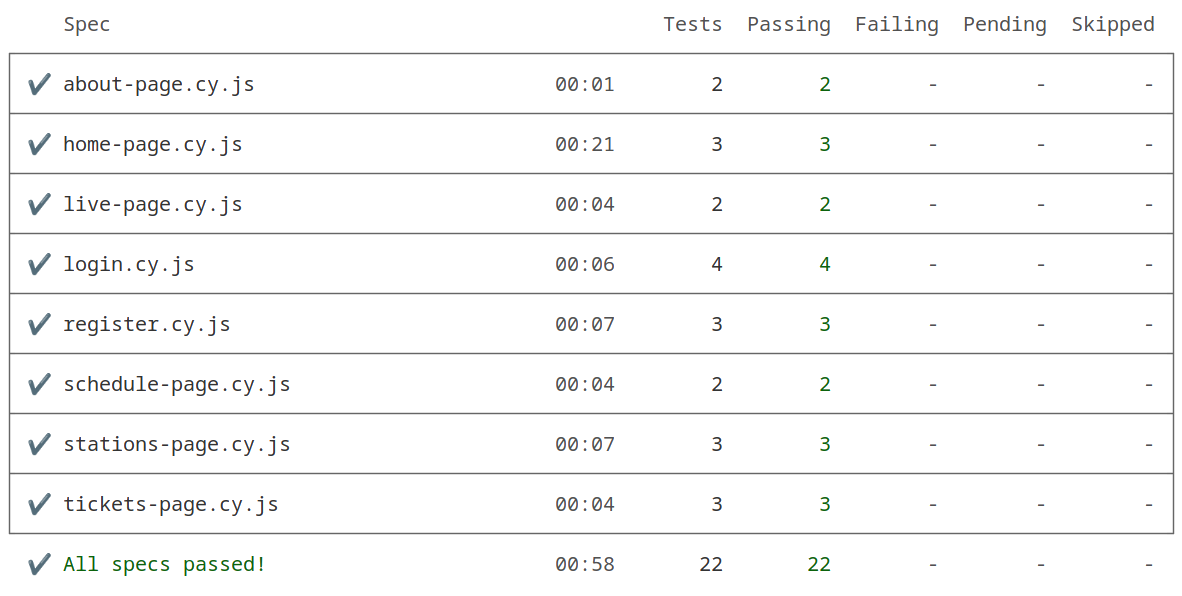
\includegraphics[width=\textwidth]{figures/cypress-user.png}
    \caption{A felhasználói weboldal tesztjei}
    \label{fig:cypress-user}
\end{figure}

Vegyünk egy példát a végponttól-végpontig tartó tesztre, amely az admin felületen történő megálló létrehozásának és törlésének működését ellenőrzi. A teszt során a következő lépések hajtódnak végre:
\begin{itemize}
  \item Bejelentkezés az admin felületre.
  \item Megállók oldal felkeresése.
  \item Kattintás a megálló hozzáadása gombra.
  \item Várakozás a térkép betöltődésére.
  \item A térképen egy pont kiválasztása, ahol a megálló létre lesz hozva.
  \item A megálló nevének megadása és a mentés gomb megnyomása.
  \item Ellenőrzés, hogy a megálló sikeresen létrejött-e.
  \item Kattintás a megálló törlése gombra.
  \item Ellenőrzés, hogy a megálló sikeresen törölve lett-e.
\end{itemize}
A teszthez tartozó programkód a következőképpen néz ki:

\begin{lstlisting}[language=JavaScript]
  it("add new station and remove it", () => {
    cy.intercept("GET", "https://api.mapbox.com/map-sessions/v1*").as("map");
    cy.login();
    cy.visit("/stations");
    cy.get(".d-flex > .v-btn").click();
    cy.wait("@map");
    cy.get(".mapboxgl-canvas").click(320, 500);
    cy.get("input[name='name']").type("test station");
    cy.get("button[type='submit']").click();
    cy.get(".v-snackbar__content").contains("Station created");
    cy.get(".v-list > .v-list-item").contains("test stat").parent().siblings().find("button").click();
    cy.get(".v-snackbar__content").contains("Station deleted");
    cy.get(".v-list > .v-list-item").should("not.contain", "test station");
  });
\end{lstlisting}

\section{Automatizált tesztelés}
A tesztek futtatásának automatizálását a GitHub Actions segítségével valósítottam meg. A GitHub Actions egy olyan funkció a GitHubon, amely lehetővé teszi előre definiált feladatok automatikus végrehajtását a kód változásának alkalmával. A Cypress biztosít egy előre megírt GitHub Actions konfigurációt, amelyet csak be kell állítani a projektünkben, és a tesztek automatikusan lefutnak minden egyes változtatás után. Az én esetemben 2 ilyen feladatra van szükség: az egyik a felhasználói, míg a másik az admin weboldal tesztjeinek futtatására. Ezekhez hozzáadtam még egy extra lépést, amely hiba esetén lementi a tesztek által készített képernyőképeket utólagos elemzés céljából. Mindhárom tesztelési feladat a "Cypress tests" nevű Action része, amelynek konfigurációs kódja a következő:
\begin{lstlisting}
name: Cypress tests
on: push
jobs:
  cypress-run:
    name: Cypress run
    runs-on: ubuntu-24.04
    steps:
      - name: Checkout
        uses: actions/checkout@v4
      - name: Cypress test USER
        uses: cypress-io/github-action@v6
        env:
          VITE_MAPBOX_TOKEN: ${{ secrets.VITE_MAPBOX_TOKEN }}
        with:
          start: npm run dev
          working-directory: USER_WEB
      - name: Cypress test ADMIN
        uses: cypress-io/github-action@v6
        env:
          VITE_MAPBOX_TOKEN: ${{ secrets.VITE_MAPBOX_TOKEN }}
        with:
          start: npm run dev
          working-directory: ADMIN_WEB
      - name: Upload screenshots
        uses: actions/upload-artifact@v4
        if: failure()
        with:
          name: cypress-screenshots
          path: |
            USER_WEB/cypress/screenshots
            ADMIN_WEB/cypress/screenshots
\end{lstlisting}

A tesztek lefutása után a GitHub Actions értesítést küld az eredményekről email-ben, és a webfelületen is megjeleníti ezeket táblázatos formában. Itt amennyiben szükséges, vissza lehet nézni a naplót vagy le lehet tölteni a hibákról készült képernyőképeket, amelyek segítségével könnyen meg lehet tudni, hogy mi okozta az esetleges hibákat. A sikeres tesztek lefutása után megjelenő összefoglaló táblázat a \ref{fig:github-actions} ábrán látható.

\begin{figure}[H]
    \centering
    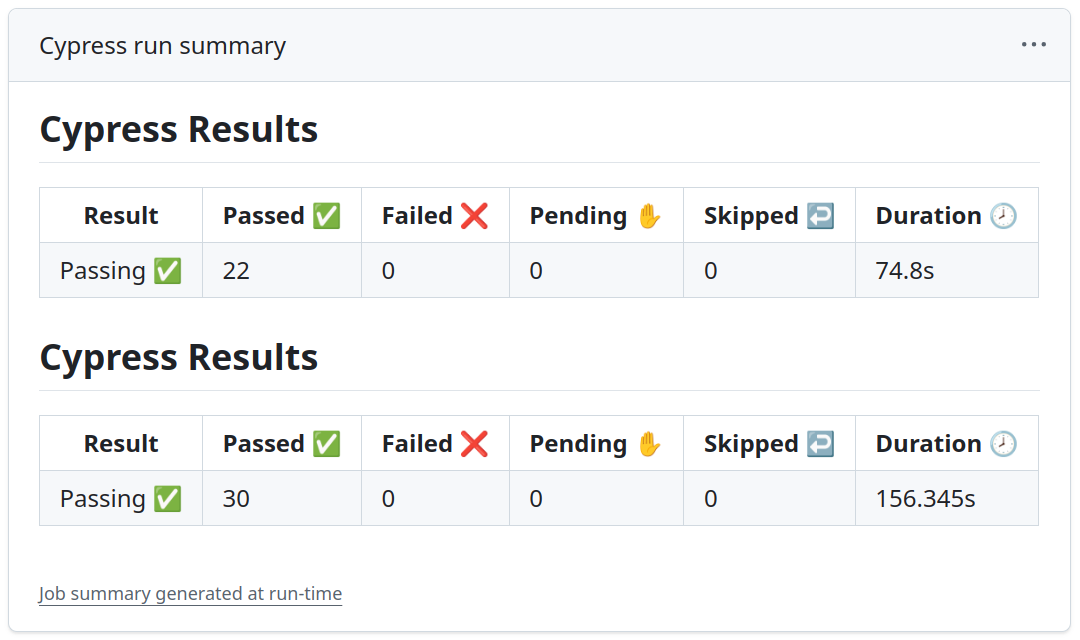
\includegraphics[width=1\textwidth]{figures/cypress-passed.png}
    \caption{A GitHub Actions által generált teszteredmények}
    \label{fig:github-actions}
\end{figure}